%!TEX root = main.tex



\begin{figure*}
\begin{smaller}
    \centering
       \hspace{-0.5cm}
        \begin{subfigure}[b]{0.4\textwidth}
        	        \centering
                    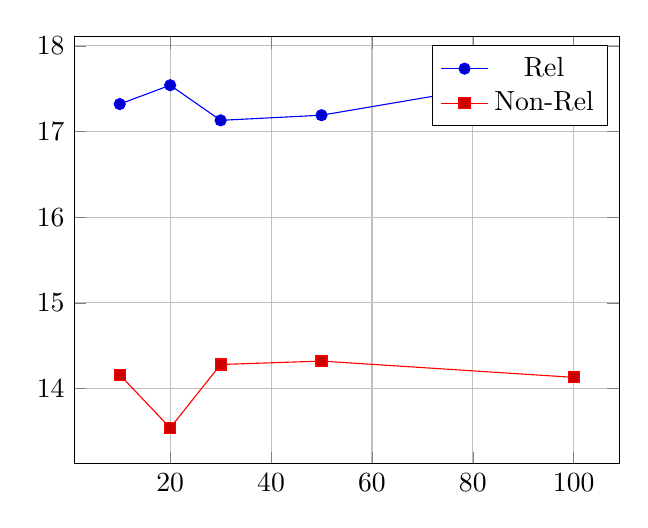
\begin{tikzpicture}
        	\begin{axis}[
        		height=7cm,
        		width=8.5cm,
        		grid=major,
        	]
        	\addplot coordinates {
        		(10,17.32)
        		(20,17.54)
        		(30,17.13)
        		(50,17.19)
        		(100,17.69)
        	};
        	\addlegendentry{Rel}
        			
        	\addplot coordinates {
        		(10,	14.16)
        		(20,	13.54)
        		(30,	14.28)
        		(50,	14.32)
        		(100,	14.13)
        		
        	};
        	\addlegendentry{Non-Rel}
        
        
        	\end{axis}
        	
        \end{tikzpicture}
        \caption{Urls}
        \label{Urls}
        \end{subfigure}
		~
		\hspace{1.5cm}
        \begin{subfigure}[b]{0.4\textwidth}
        	        \centering
                    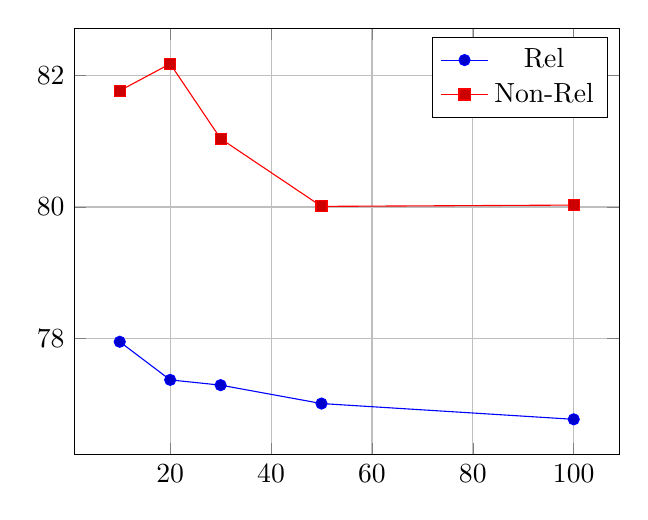
\begin{tikzpicture}
        	\begin{axis}[
        		height=7cm,
        		width=8.5cm,
        		grid=major,
        	]
        	\addplot coordinates {
        	(10,77.95)
        	(20,77.37)
        	(30,77.29)
        	(50,77.01)
        	(100,76.77)
        	};
        	\addlegendentry{Rel}
        			
        	\addplot coordinates {
        		(10,	81.77)
        		(20,	82.18)
        		(30,	81.04)
        		(50,	80.01)
        		(100,	80.03)
        	};
        	\addlegendentry{Non-Rel}
        
        
        	\end{axis}
        	
        \end{tikzpicture}
        \caption{Text}
        \label{Text}
        \end{subfigure}
\end{smaller}
\caption{Rate (\%) of space dedicated to Urls and Text in Relevant and Non-Relevant documents at different cut-off points.}
\label{urltext}
\vspace{0.5cm}
\end{figure*}






